\section{Background}

\section{Approach}

\subsection{Motivation}

\begin{figure}
    \centering
    \begin{subfigure}[b]{0.375\textwidth}
        \centering
        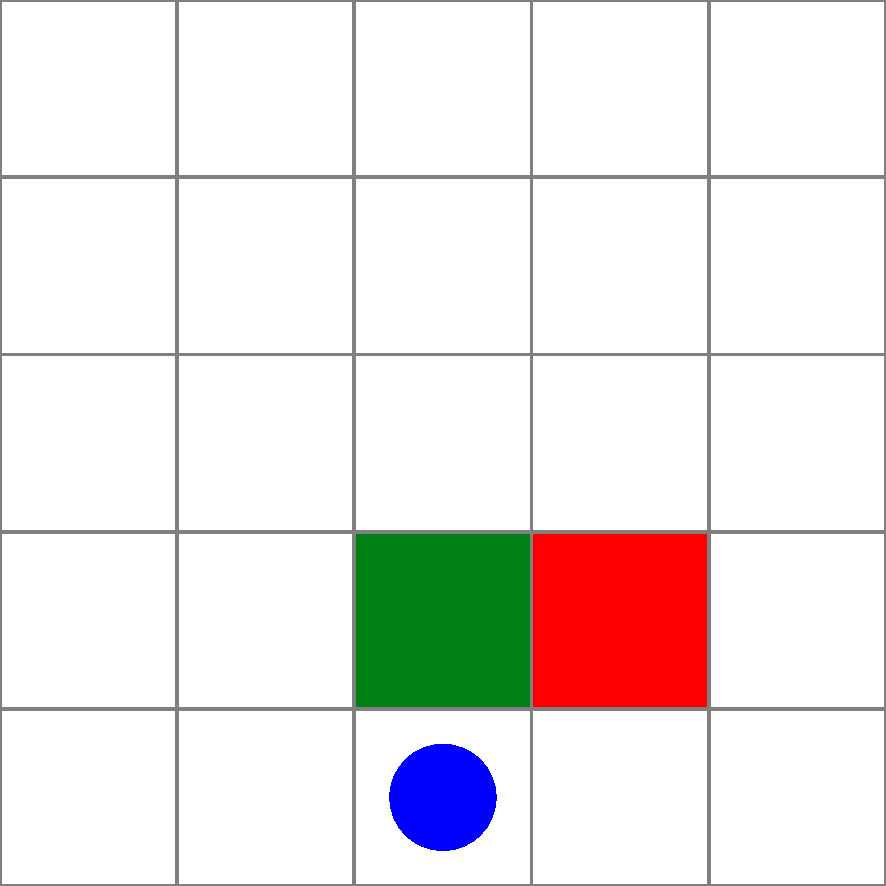
\includegraphics[width=\textwidth]{figures/iterative_validation/gridworld1.pdf}
        \caption{Reference MDP}    
        \label{fig:ivm_base}
    \end{subfigure}
    \hfill
    \begin{subfigure}[b]{0.375\textwidth}  
        \centering 
        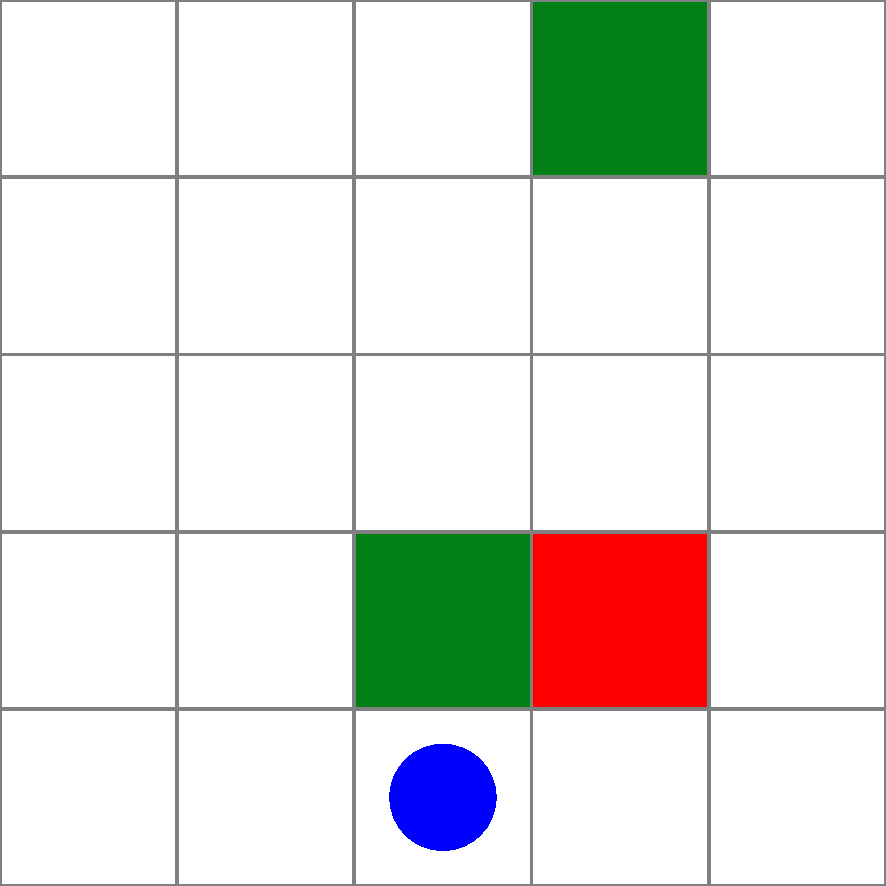
\includegraphics[width=\textwidth]{figures/iterative_validation/gridworld2.pdf}
        \caption{Locally similar}  
        \label{fig:ivm_locally_optimal}
    \end{subfigure}
    \vskip\baselineskip
    \begin{subfigure}[b]{0.375\textwidth}   
        \centering 
        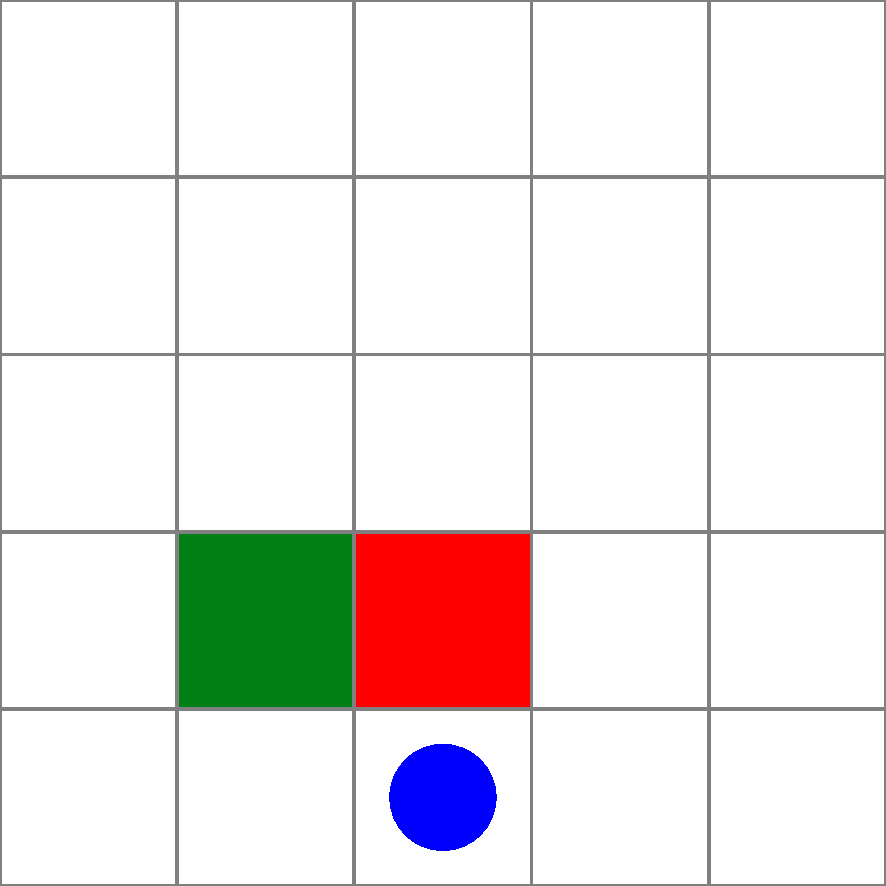
\includegraphics[width=\textwidth]{figures/iterative_validation/gridworld3.pdf}
        \caption{Translation}  
        \label{fig:ivm_translation}
    \end{subfigure}
    \hfill
    \begin{subfigure}[b]{0.375\textwidth}   
        \centering 
        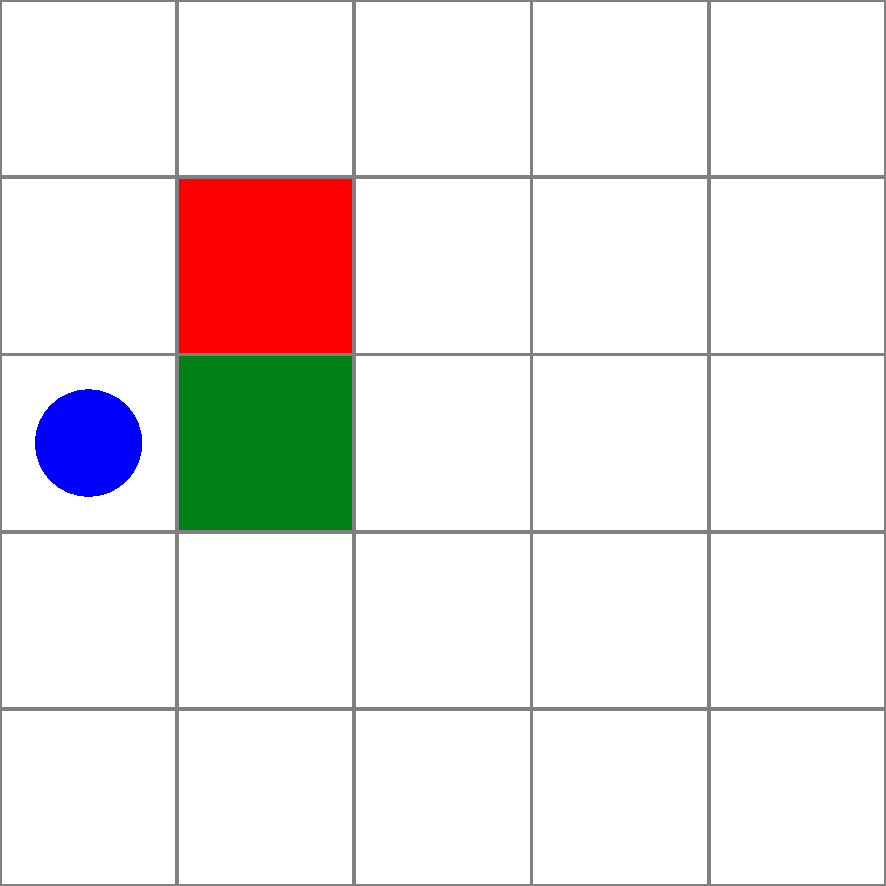
\includegraphics[width=\textwidth]{figures/iterative_validation/gridworld4.pdf}
        \caption{Rotations}
        \label{fig:ivm_rotation}
    \end{subfigure}
    \caption{Scenarios where policy transfer from a reference solution should be feasible.}
    \label{fig:ivm}
\end{figure}

\section{Network Architecture}
\begin{figure}[!t]
\centering
 \begin{subfigure}[b]{0.475\textwidth}
    % TikZ diagram for black-box safety validation problem formulation.
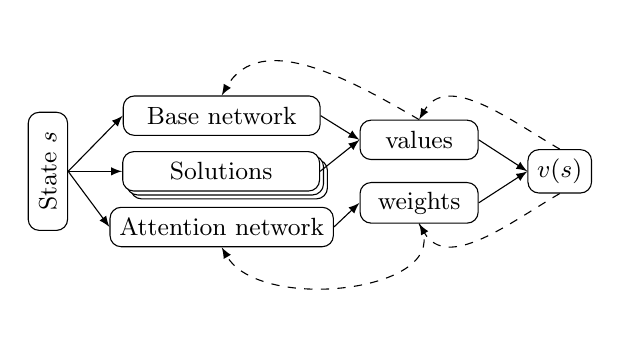
\begin{tikzpicture}
    \tikzstyle{every node}=[font=\small, align=center]
    \tikzset{
        n/.style={draw, rounded corners, minimum height=0.5cm, minimum width = 1.5cm},
        n2/.style={n, minimum width=2.5cm}
        }
    
    %state 
    \node (state) [n, rotate=90] {\small State $s$};
    
    %base network
    \node (base) [n2, above right of=state, xshift=1.5cm] {Base network};
    
    %Solutions
    \node (solutionsback1) [n2, right of=state, xshift=1.3cm, yshift=-0.1cm] {};
    \node (solutionsback2) [n2, fill=white, right of=state, xshift=1.25cm, yshift=-0.05cm] {};
    \node (solutions) [n2, fill=white, right of=state, xshift=1.2cm] {Solutions};
    
    %weights
    \node (attn) [n2, below right of=state, xshift=1.5cm] {Attention network};
    

    \node (values) [n, below right of=base, xshift=1.8cm, yshift = 0.4cm] {values};
    
     \node (weights) [n, above right of=attn, xshift=1.8cm, yshift = -0.4cm] {weights};
     
     \node (pfail) [n, minimum width = 0.5cm, right of=state, xshift=5.5cm] {$v(s)$};
    

    \draw[-latex] (state.south) -- (base.west);
    \draw[-latex] (state.south) -- (solutions.west);
    \draw[-latex] (state.south) -- (attn.west);
    
    \draw[-latex] (base.east) -- (values.west);
    \draw[-latex] (solutions.east) -- (values.west);
    \draw[-latex] (attn.east) -- (weights.west);
    
    \draw[-latex] (weights.east) -- (pfail.west);
    \draw[-latex] (values.east) -- (pfail.west);
    
    
    % backprop
    
    \draw [dashed, -latex] (weights.south) to [out=-1500,in=-60] (attn.south);
    \draw [dashed, -latex] (pfail.south) to [out=-150,in=-60] (weights.south);
    \draw [dashed, -latex] (values.north) to [out=150,in=60] (base.north);
    \draw [dashed, -latex] (pfail.north) to [out=150,in=60] (values.north);
\end{tikzpicture}
    \caption{The A2T network. Dashed lines represent backpropagation for learning parameters.}
    \label{fig:A2T_Network}
    \end{subfigure}
    \hfill
    \begin{subfigure}[b]{0.475\textwidth}
        % TikZ diagram for black-box safety validation problem formulation.
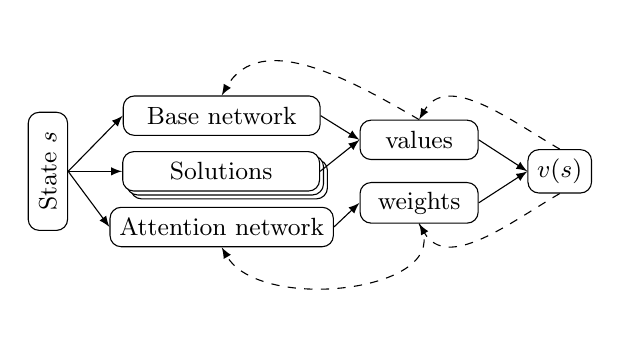
\begin{tikzpicture}
    \tikzstyle{every node}=[font=\small, align=center]
    \tikzset{
        n/.style={draw, rounded corners, minimum height=0.5cm, minimum width = 1.5cm},
        n2/.style={n, minimum width=2.5cm}
        }
    
    %state 
    \node (state) [n, rotate=90] {\small State $s$};
    
    %base network
    \node (base) [n2, above right of=state, xshift=1.5cm] {Base network};
    
    %Solutions
    \node (solutionsback1) [n2, right of=state, xshift=1.3cm, yshift=-0.1cm] {};
    \node (solutionsback2) [n2, fill=white, right of=state, xshift=1.25cm, yshift=-0.05cm] {};
    \node (solutions) [n2, fill=white, right of=state, xshift=1.2cm] {Solutions};
    
    %weights
    \node (attn) [n2, below right of=state, xshift=1.5cm] {Attention network};
    

    \node (values) [n, below right of=base, xshift=1.8cm, yshift = 0.4cm] {values};
    
     \node (weights) [n, above right of=attn, xshift=1.8cm, yshift = -0.4cm] {weights};
     
     \node (pfail) [n, minimum width = 0.5cm, right of=state, xshift=5.5cm] {$v(s)$};
    

    \draw[-latex] (state.south) -- (base.west);
    \draw[-latex] (state.south) -- (solutions.west);
    \draw[-latex] (state.south) -- (attn.west);
    
    \draw[-latex] (base.east) -- (values.west);
    \draw[-latex] (solutions.east) -- (values.west);
    \draw[-latex] (attn.east) -- (weights.west);
    
    \draw[-latex] (weights.east) -- (pfail.west);
    \draw[-latex] (values.east) -- (pfail.west);
    
    
    % backprop
    
    \draw [dashed, -latex] (weights.south) to [out=-1500,in=-60] (attn.south);
    \draw [dashed, -latex] (pfail.south) to [out=-150,in=-60] (weights.south);
    \draw [dashed, -latex] (values.north) to [out=150,in=60] (base.north);
    \draw [dashed, -latex] (pfail.north) to [out=150,in=60] (values.north);
\end{tikzpicture}
        \caption{The A2T network. Dashed lines represent backpropagation for learning parameters.}
        \label{fig:A2T_Network}
    \end{subfigure}
\end{figure}

\section{Experiments}

\begin{figure}
    \centering
    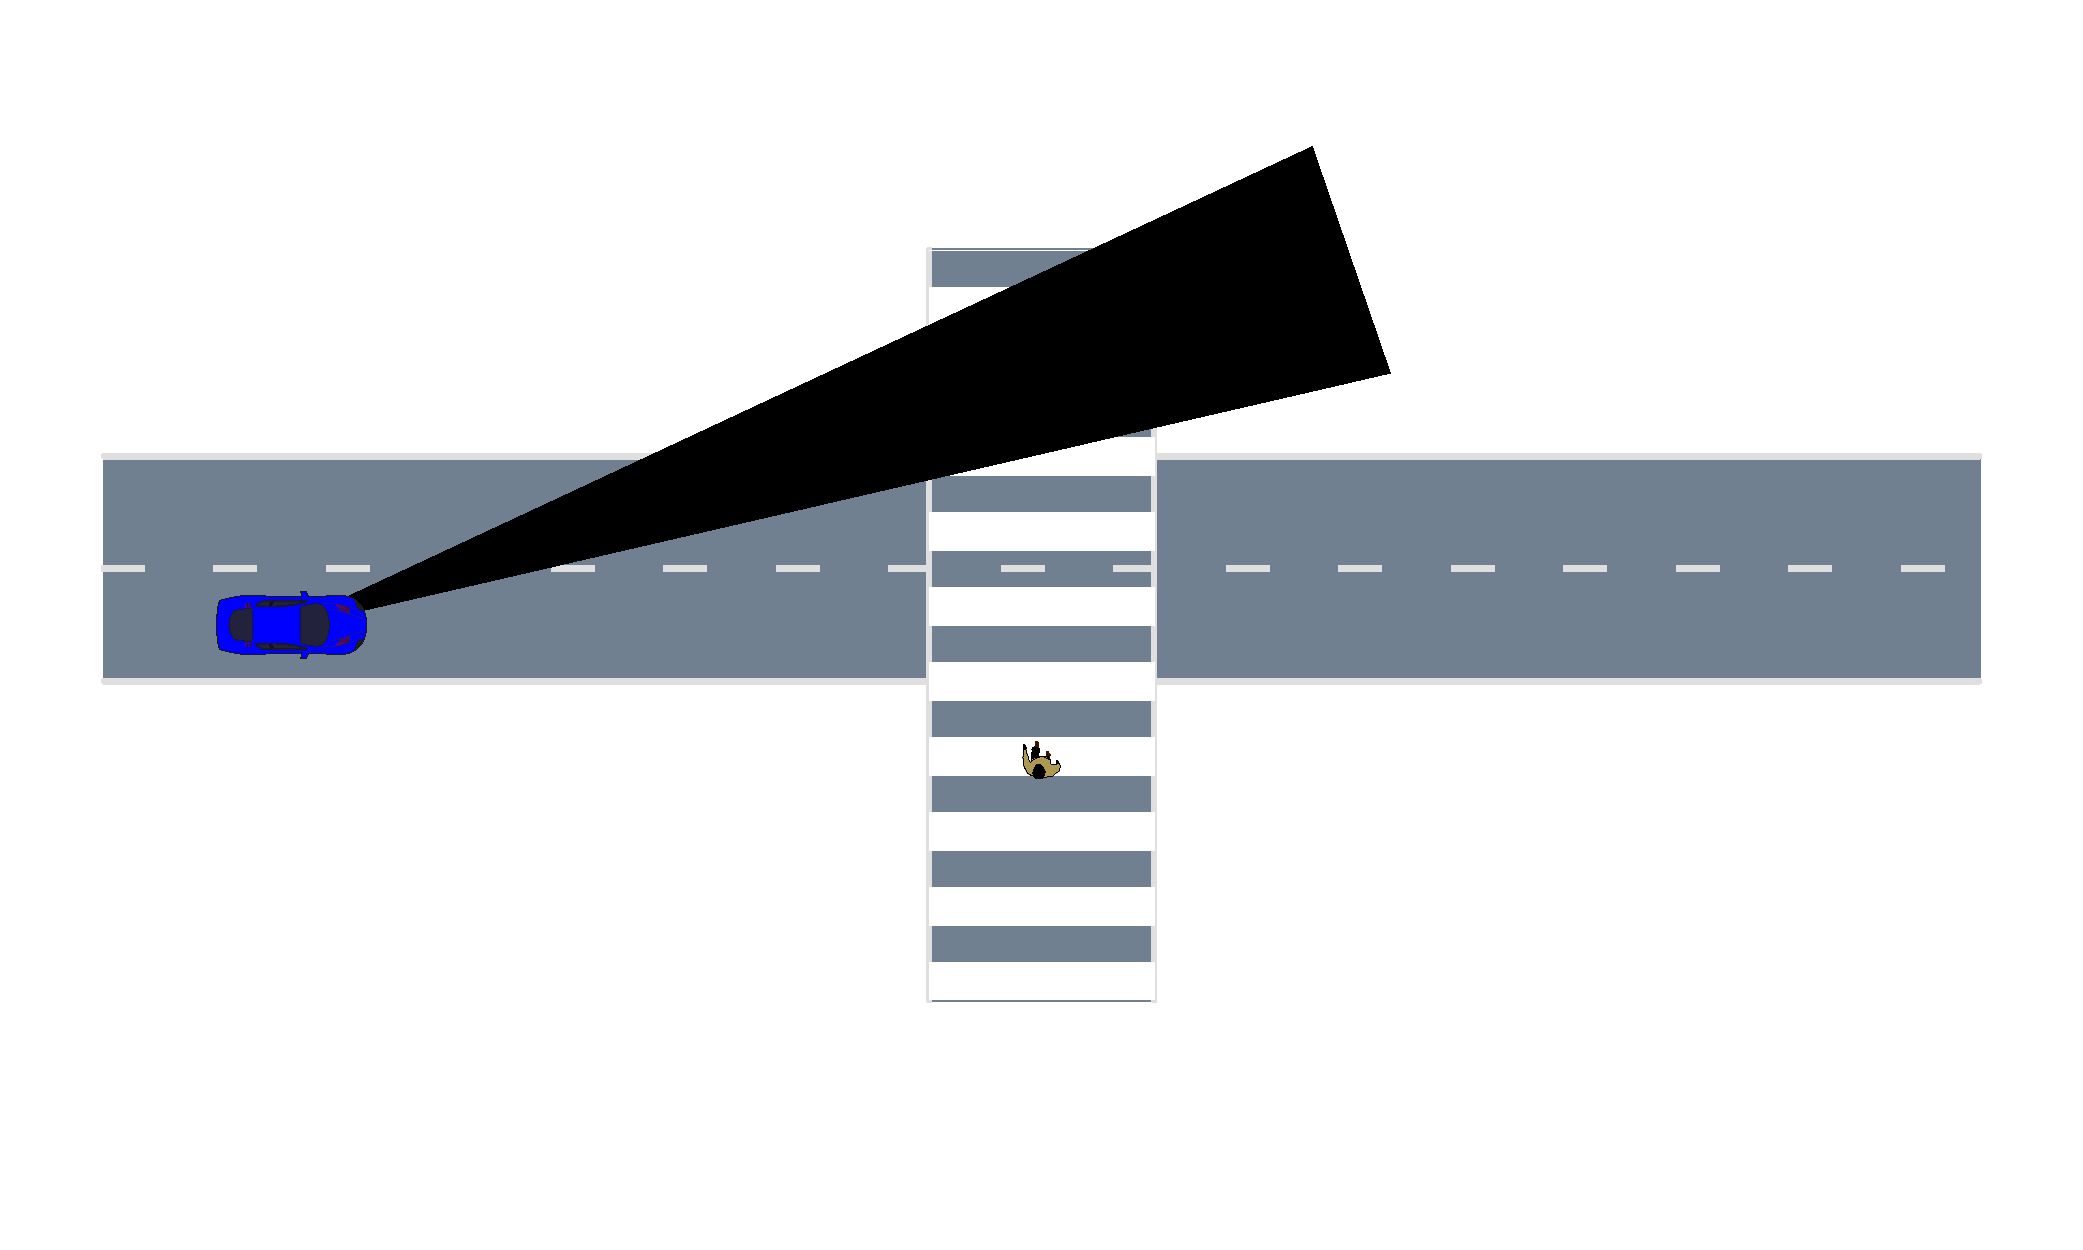
\includegraphics[width=0.7\textwidth]{figures/iterative_validation/blindspot.pdf}
    \caption{Autonomous vehicle with forward-facing blindspot}
    \label{fig:ivm_blindspot}
\end{figure}

\begin{figure}
    \centering
    \begin{subfigure}[b]{0.6\textwidth}
        \centering
        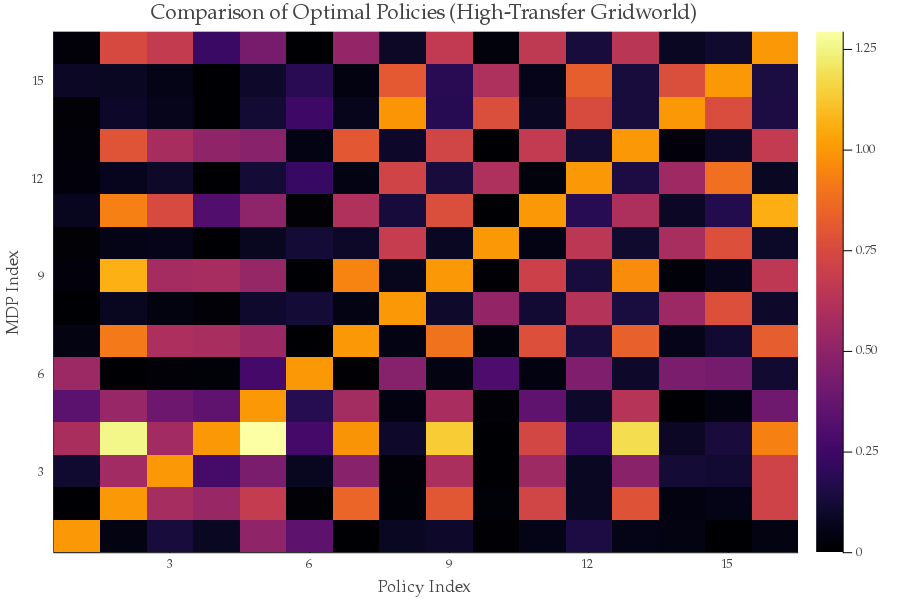
\includegraphics[width=\textwidth]{figures/iterative_validation/high_transfer_heatmap.png}  
        \caption{High-Transfer Gridworld}    
        \label{fig:ivm_base}
    \end{subfigure}
    \vskip\baselineskip
    \begin{subfigure}[b]{0.6\textwidth}  
        \centering 
        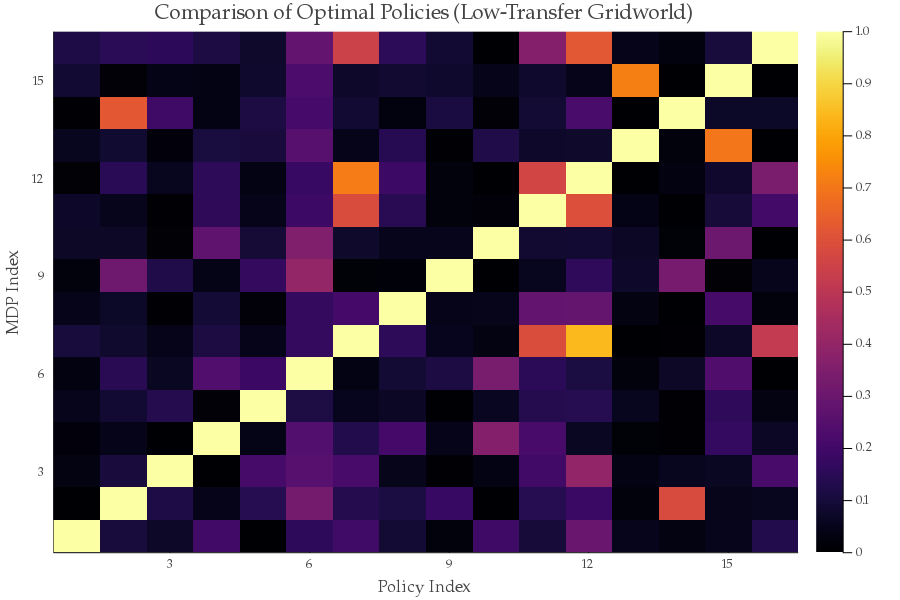
\includegraphics[width=\textwidth]{figures/iterative_validation/low_transfer_heatmap.png}
        \caption{Low-Transfer Gridworld}  
        \label{fig:ivm_locally_optimal}
    \end{subfigure}
    \vskip\baselineskip
    \begin{subfigure}[b]{0.6\textwidth}  
        \centering 
        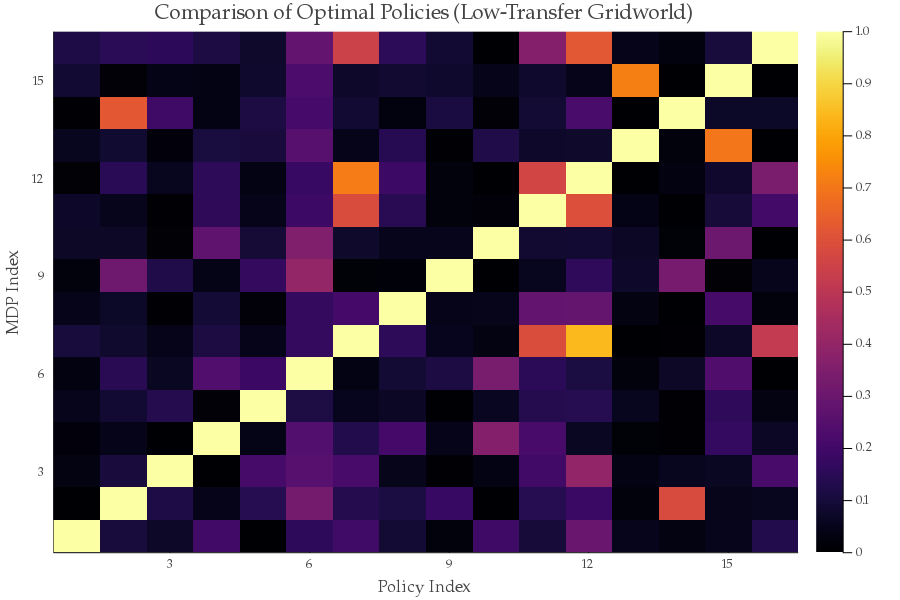
\includegraphics[width=\textwidth]{figures/iterative_validation/low_transfer_heatmap.png}
        \caption{Autonomous Vehicle}  
        \label{fig:ivm_locally_optimal}
    \end{subfigure}
\end{figure}

\section{Discussion}

% Literature review
% Transfer learning in reinforcement learning domains: a survey
\cite{taylor2009transfer}
% Identify good baselines
% Summarize a variety of approaches for transfer

The evaluation of the algorithms will be from \emph{jumpstart} which is the initial safety validation performance on the new task, \emph{asymptotic performance} which is the safety validation performance with reference tasks, and \emph{steps to threshold} which is the number of training steps require to reach a specified level of performance.

We use the number of training steps rather than the wall clock time because we assume that, in practice, the cost of running the simulator is much large than the cost of updating the parameters of the model. This is a good assumption for high-fidelity simulators that are typical for cyber-physical systems.

By the nature of the safety-validation use case, we assume that previous tasks arrive one at a time, and we need to solve the current task before having access to the next tasks. This precludes the use of Meta-Learning or Multi-task approaches which simultaneously train on a distribution of different tasks. 


We assume that the training time of previous source tasks is a sunk cost and it is not included in the number of steps to threshold for the transfer learning algorithms. This assumption is valid in the case of iterative safety validation, because version of the system must be validated regardless of the approach used. 


\cite{lazaric2012transfer}
When the state or action spaces change, then a state or action mapping needs to be defined. Previous approaches use expert knowledge to define the mapping~\cite{taylor2007transfer}, while some other approaches learn the mapping directly~\cite{taylor2008autonomous}. 


\cite{rajendran2017attend}. A2T combines the solutions of $m$ problems with a solution learned from scratch $v_{\rm base}$ using a learned set of state-dependent attention weights $w(s)$. The estimated probability of failure for a state $s$, $\tilde{v}(s)$, is then given by 
\begin{equation}
\tilde{v}(s) = w_0(s) v_{\rm base}(s) + \sum_{i=1}^m w_i(s) v_i(s^{(i)}) \label{eq:A2T}
\end{equation}
where $w_i$ and $v_{\rm base}$ have parameters that can be learned.

The use of attention weights allows A2T to learn which solutions are most relevant in which states. If none of the subproblems are providing a good estimate then the base network will learn a good estimate from scratch.


